\documentclass{article}%
\usepackage[T1]{fontenc}%
\usepackage[utf8]{inputenc}%
\usepackage{lmodern}%
\usepackage{textcomp}%
\usepackage{lastpage}%
\usepackage[head=40pt,margin=0.5in,bottom=0.6in]{geometry}%
\usepackage{graphicx}%
%
\title{\textbf{Unión Europea espera que Gobierno de Maduro "reconsidere" decisión de expulsar a embajador alemán}}%
\author{AFP}%
\date{07/03/2019}%
%
\begin{document}%
\normalsize%
\maketitle%
\textbf{URL: }%
http://www.eluniversal.com/politica/34976/union{-}europea{-}espera{-}que{-}gobierno{-}de{-}maduro{-}reconsidere{-}decision{-}de{-}expulsar{-}a{-}embajador{-}aleman\newline%
%
\textbf{Periodico: }%
EU, %
ID: %
34976, %
Seccion: %
politica\newline%
%
\textbf{Palabras Claves: }%
NO\_TIENE\newline%
%
\textbf{Derecho: }%
2.1%
, Otros Derechos: %
\newline%
%
\textbf{\textit{"Lamentamos el hecho de que el embajador alemán en Venezuela se vea obligado a abandonar el país en un contexto político tenso y complejo", dijo la vocera de la diplomacia europea, Maja Kocijancic}}%
\newline%
\newline%
%
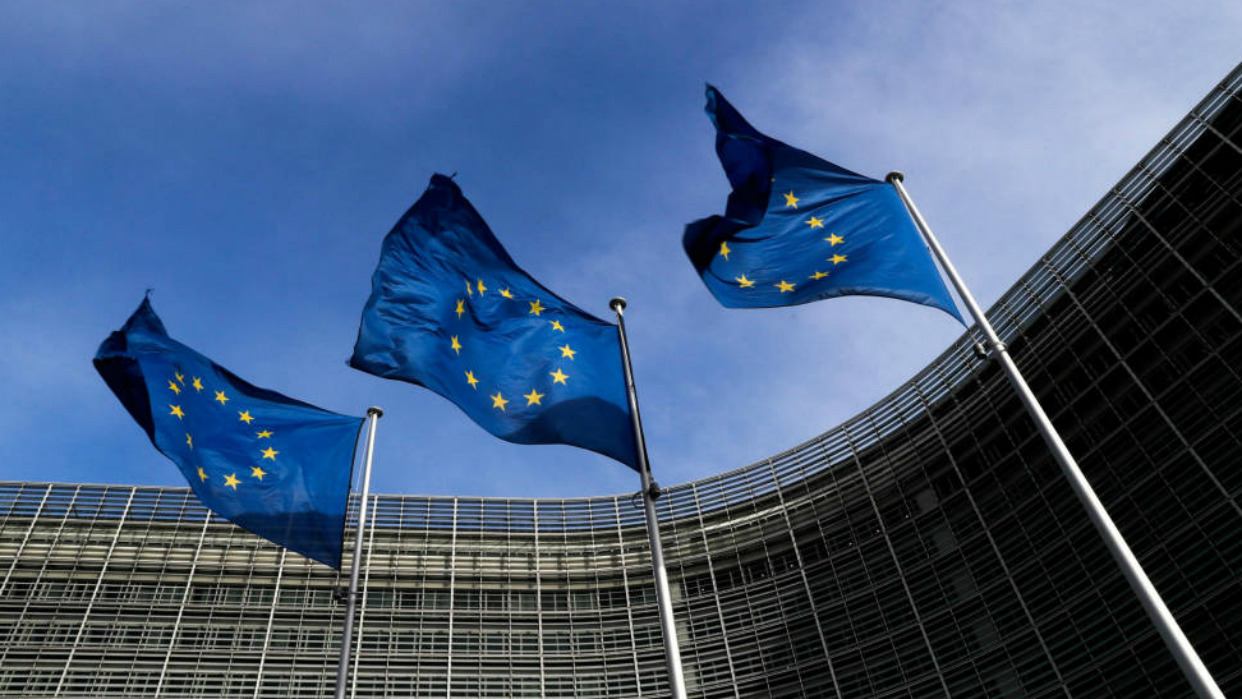
\includegraphics[width=300px]{EU_34976.jpg}%
\newline%
%
Bruselas.{-} La Unión Europea (UE) lamentó este jueves la decisión del Gobierno de Nicolás Maduro de expulsar al embajador alemán del país y dijo esperar que Caracas lo "reconsidere".%
\newline%
%
"Lamentamos el hecho de que el embajador alemán en Venezuela se vea obligado a abandonar el país en un contexto político tenso y complejo", dijo en rueda de prensa la vocera de la diplomacia europea, Maja Kocijancic.%
\newline%
%
Tras recordar que los europeos quieren mantener "las líneas de comunicación" con todos las partes en Venezuela, incluido el gobierno, la portavoz dijo que, "desde esta perspectiva", "la UE espera que se reconsidere" la decisión.%
\newline%
%
El Gobierno de Maduro ordenó el miércoles al embajador alemán, Daniel Kriener, abandonar el país en 48 horas por "recurrentes actos de injerencia en los asuntos internos", por su respaldo al líder opositor Juan Guaidó.%
\newline%
%
El ministro alemán de Relaciones Exteriores, Heiko Maas, criticó ese día una decisión "incomprensible" que "agrava la situación y no contribuye a la distensión" y reiteró el apoyo de Alemania a Guaidó.%
\newline%
%
Alemania forma parte de la veintena de países europeos que reconocieron al opositor como presidente interino de Venezuela. Kreiner lo recibió días atrás en el aeropuerto de Caracas tras una visita a varios países sudamericanos.%
\newline%
%
La vocera europea reiteró el compromiso de la UE en hallar una "solución pacífica y democrática" a la crisis en el país, por lo que lanzó un Grupo de Contacto Internacional (GCI) "del que Alemania es un miembro activo".%
\newline%
%
\end{document}